\documentclass{article}
\usepackage[utf8]{inputenc}
\usepackage{graphicx}
\usepackage{float}
\usepackage{hyperref}
%This means that any images must be in a folder named 'images' located in the same directory as this main.tex file
\graphicspath{ {./images/} }

\title{UAS Tracking Document}
\date{September 2021}
\author{}
\begin{document}

\maketitle

\section*{Introduction}
The purpose of this document is to help record changes made to the OpenUAS so that the design can be traced back and optimized as needed. \\ \\
To add new versions or tests to this iteration of the OpenUAS, reference the UAS 1.X section of template.tex. If an entirely new design is made and needs to be documented, create a new tex file names UAS\_X where X will be the version of the UAS. To fill in information, once again reference template.tex or any other UAS.tex files.\\ \\
If you have any questions or suggestions about this document please contact Alex VandeLoo (aavande@iastate.edu)
\newpage

\tableofcontents
\newpage

%-----------------------------------------------------------------------------------------------------------------------------

%Version 1.0 Start
\addcontentsline{toc}{section}{UAS 1.0 [Veronica]}
\section*{
	\begin{center}
	UAS 1.0 [Veronica]
	\end{center}
}

\addcontentsline{toc}{subsection}{Changes Overview}
\subsection*{Changes Overview}
This is the initial version that achieved flight.

\addcontentsline{toc}{subsection}{Reasoning for Decisions}
\subsection*{Reasoning for Decisions}
N/A

\addcontentsline{toc}{subsection}{Tradeoffs}
\subsection*{Tradeoffs}
N/A

\addcontentsline{toc}{subsection}{Structure}
\subsection*{Structure}
Include a solid model of the UAS. \\

\begin{figure}[H]
	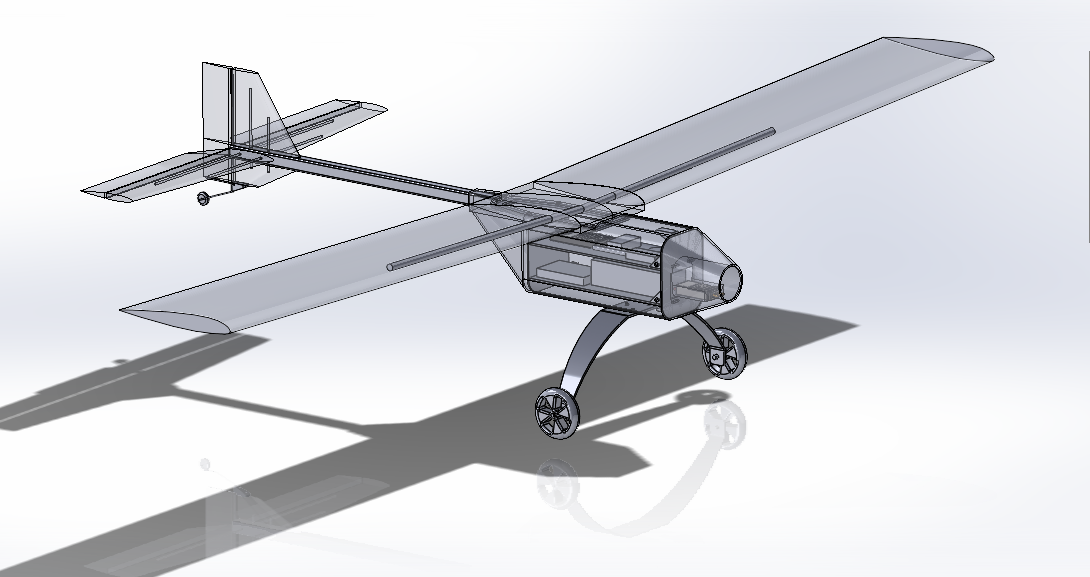
\includegraphics[width = 5cm]{UAS_1_0_SolidModel.png}
	\caption{UAS 1.0 Solidworks Model}
\end{figure}

\begin{figure}[H]
	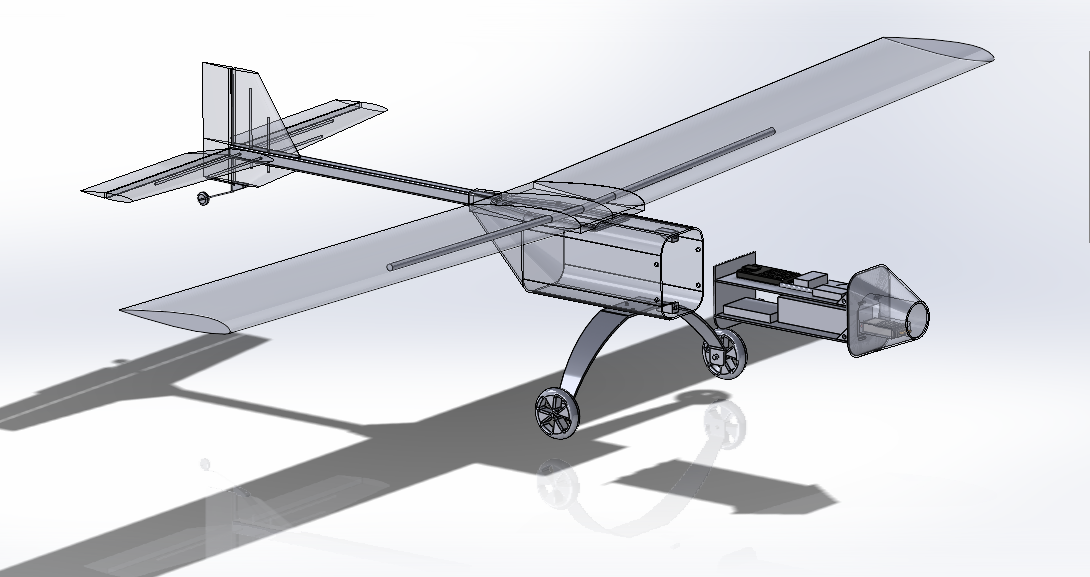
\includegraphics[width = \columnwidth]{UAS_1_0_SolidModel_ElecBay.png}
	\caption{UAS 1.0 Solidworks Model with Removed Electronics Bay}
\end{figure}

\addcontentsline{toc}{subsection}{Materials}
\subsection*{Materials}

\begin{tabular}{ c c }
	\textbf{Part of UAS} & \textbf{Material}  \\ 
	 Tail Surfaces & Foam Core, Carbon Fiber  \\  
	 Tail Beam & 3/4" Carbon Fiber Rod  \\ 
	 Fuselage & Carbon Fiber  \\  
	 Wings & Foam Core, Carbon Fiber  \\  
	 Nose Cone & Foam Core, Carbon Fiber  \\  
	 %Part of UAS & Material \\
\end{tabular} \\

\addcontentsline{toc}{subsection}{Electronics}
\subsection*{Electronics}
\subsubsection*{Wiring Diagram}
Include an image of the wiring diagram, make sure to indicate which lines are power, signal, and ground. \\ \\
\begin{figure}[H]
	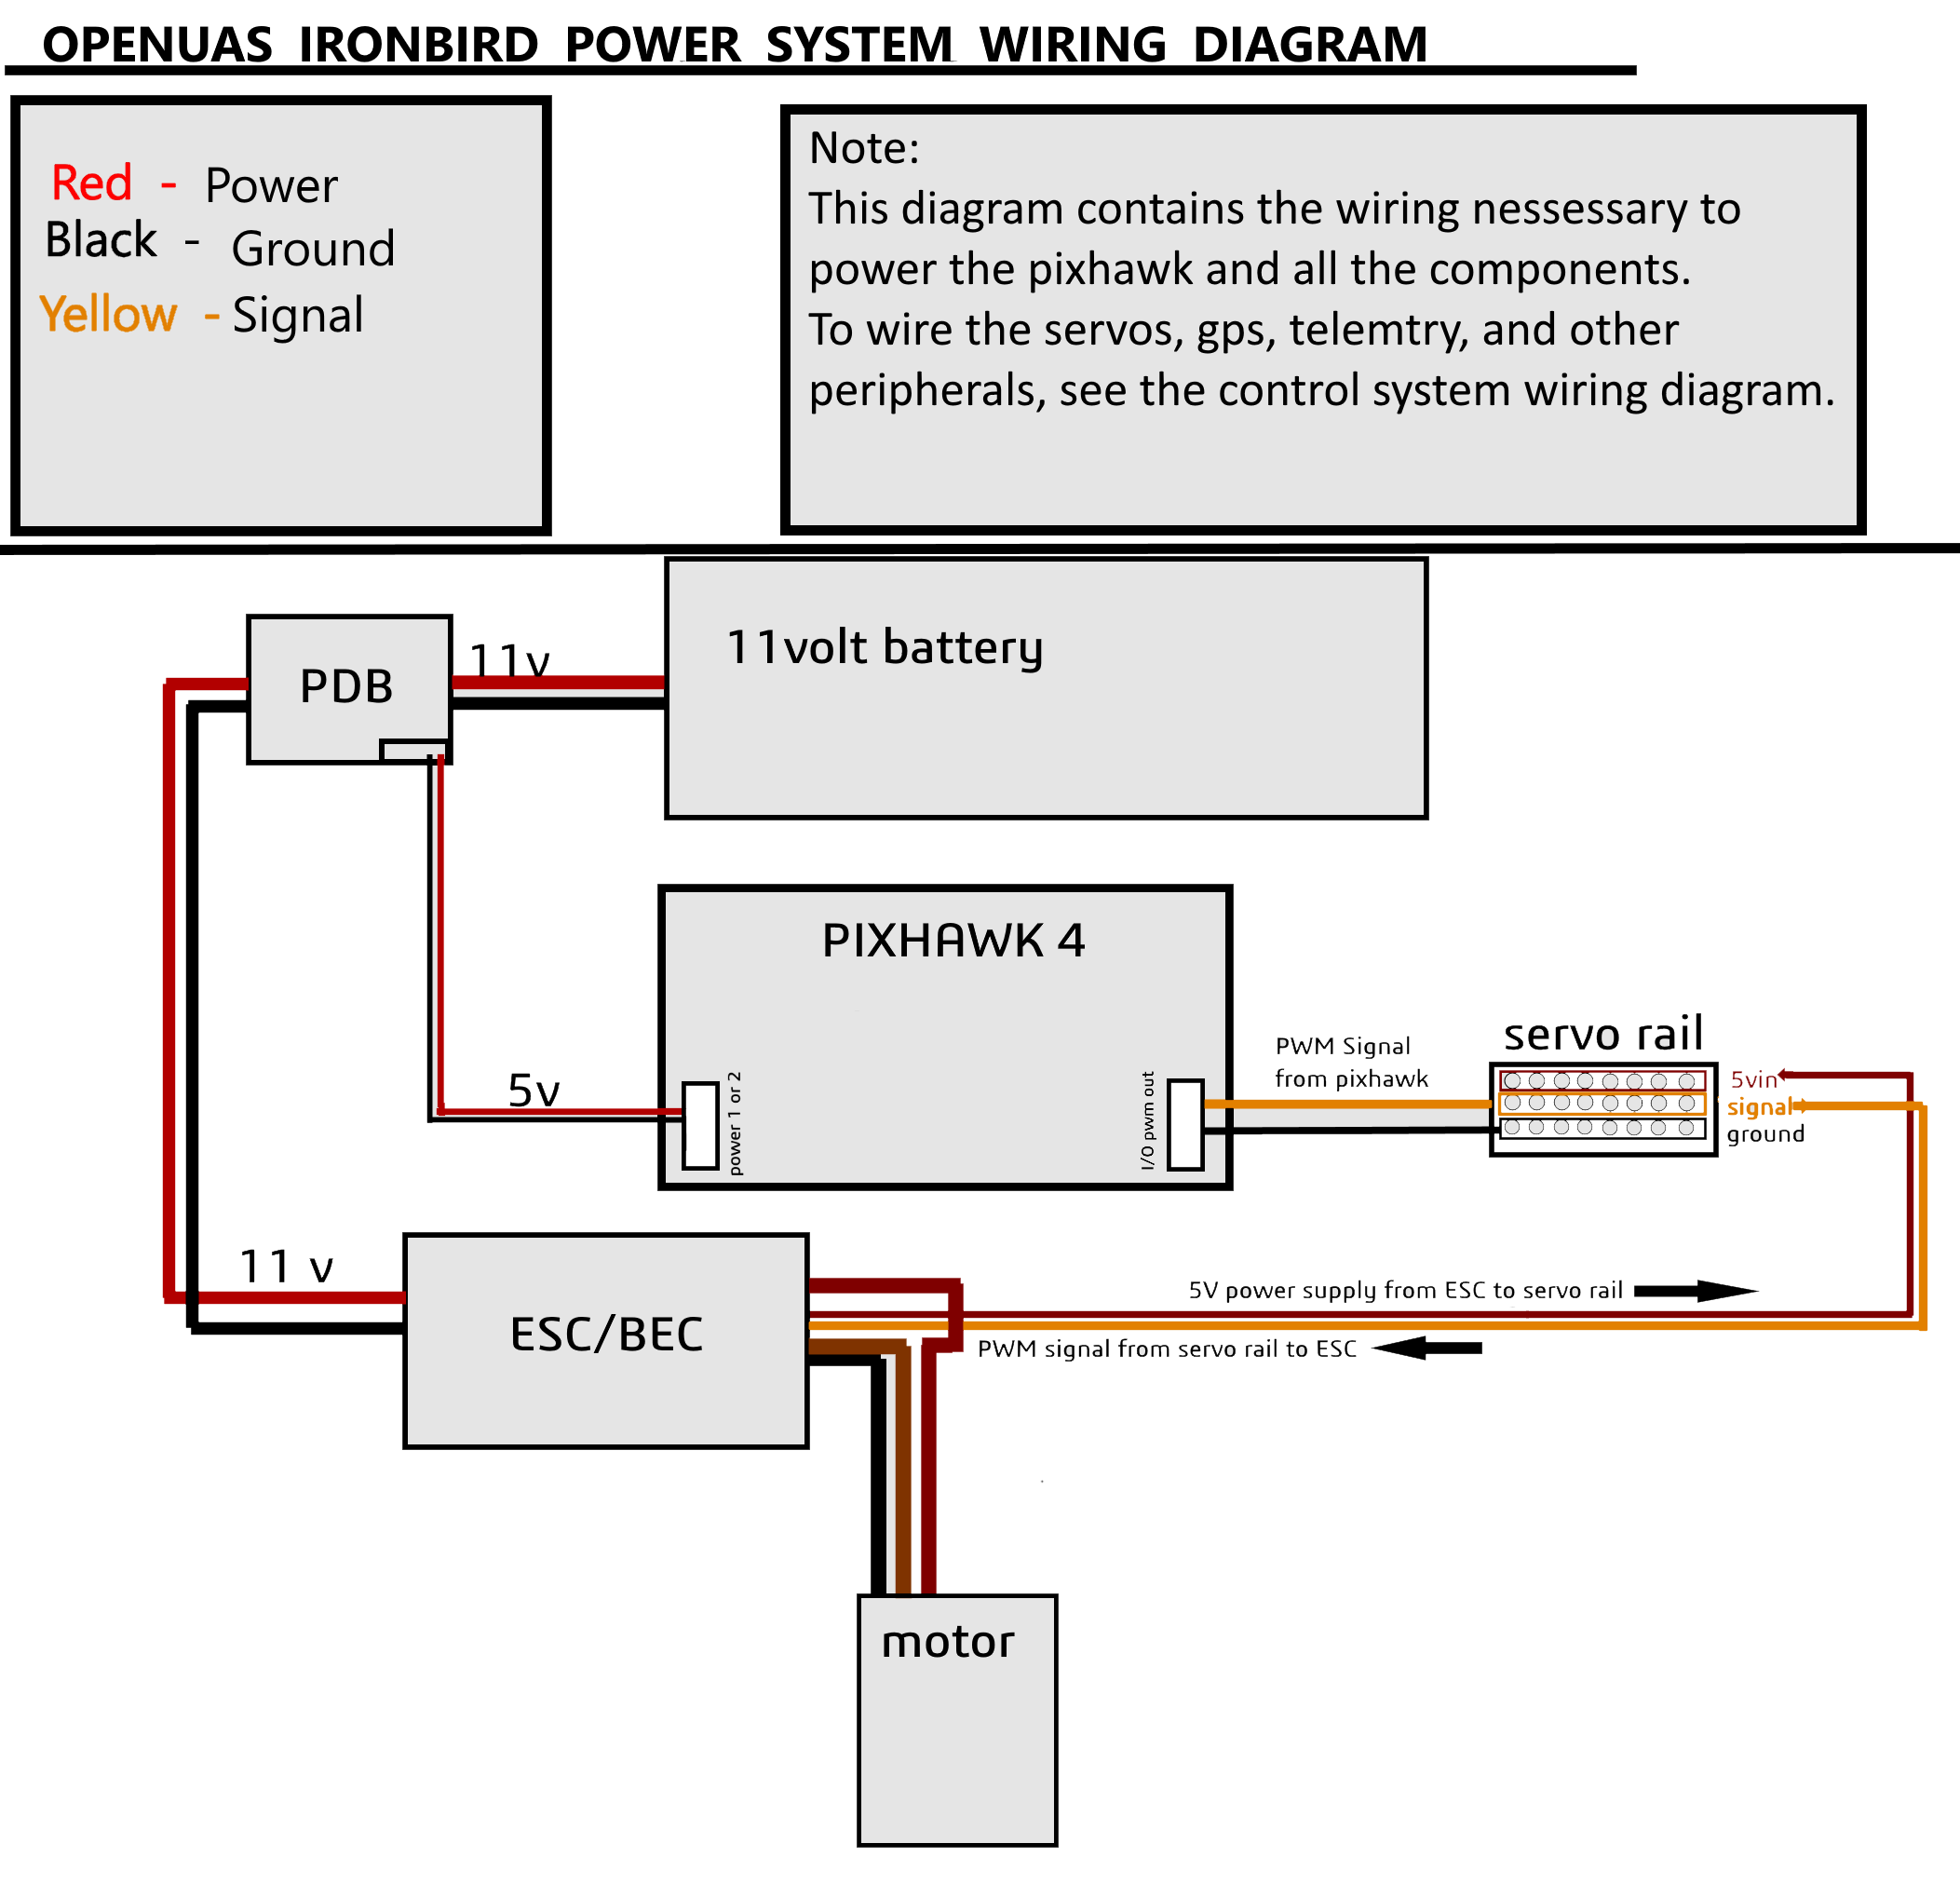
\includegraphics[width = \columnwidth]{UAS_1_0_Wiring.jpg}
	\caption{UAS 1.0 Wiring Diagram}
\end{figure}

\begin{figure}[H]
	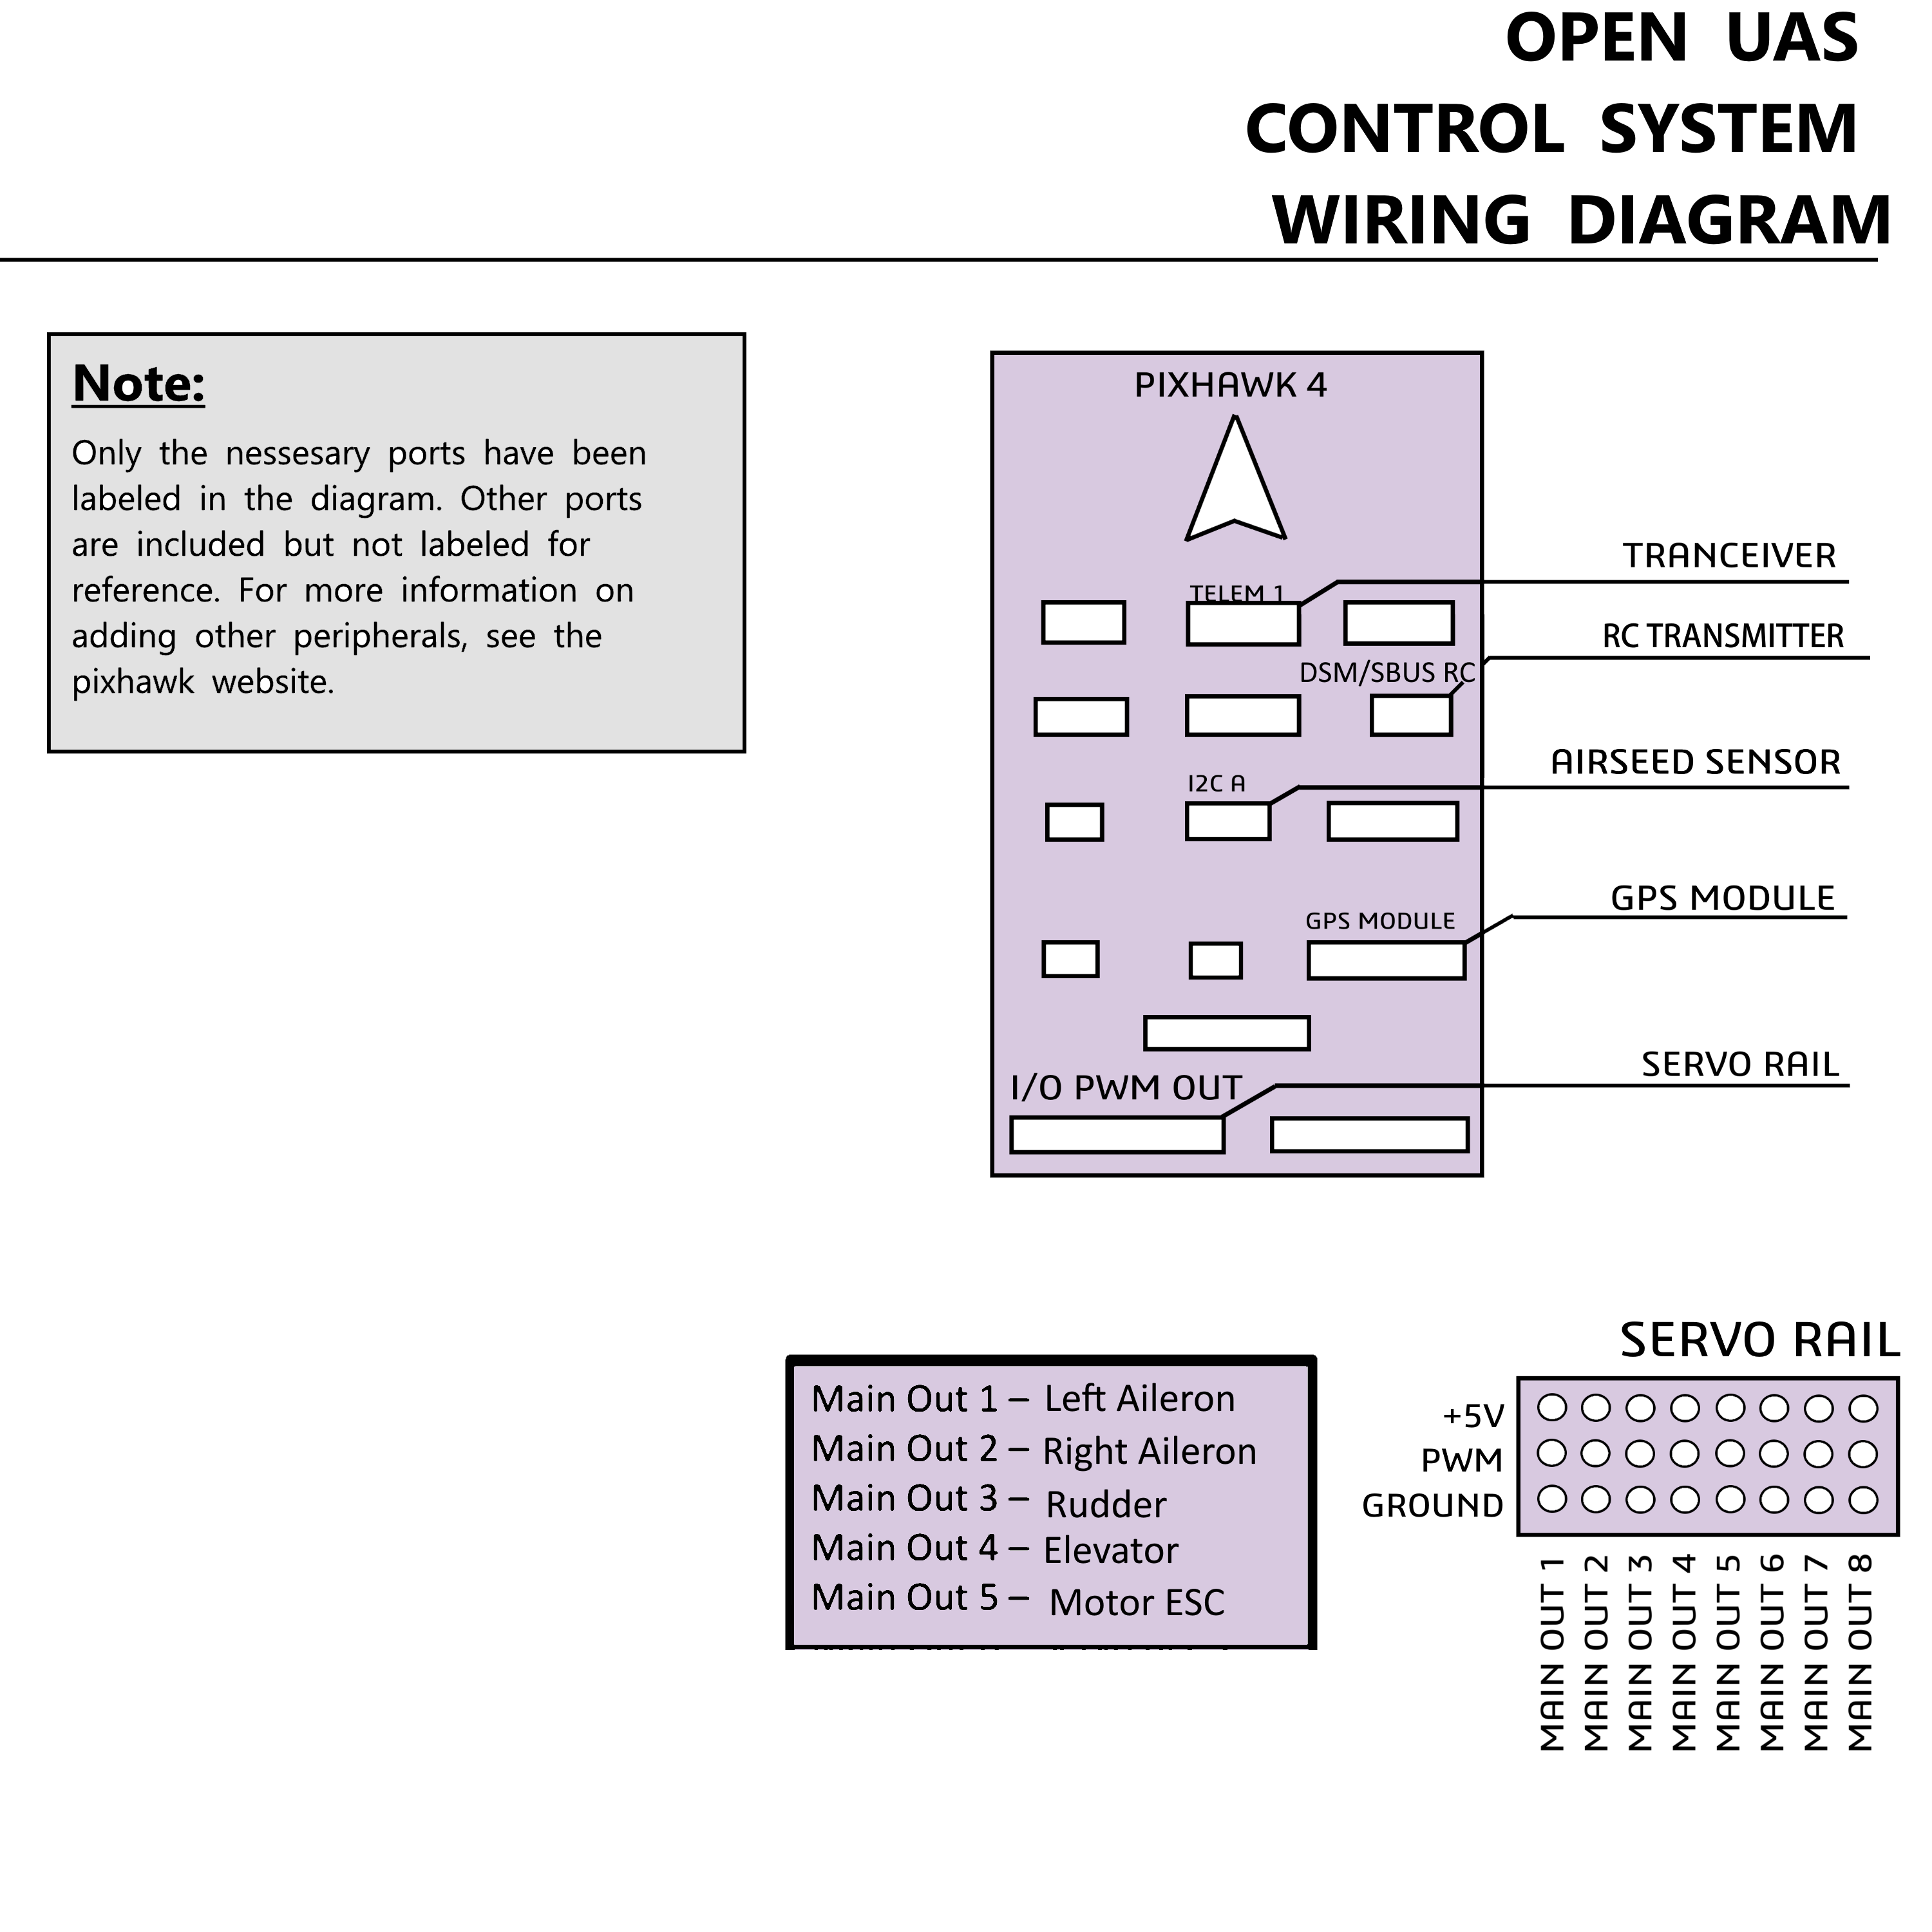
\includegraphics[width = \columnwidth]{UAS_1_0_Pixhawk.jpg}
	\caption{UAS 1.0 Pixhawk Setup}
\end{figure}


\subsubsection*{Electrical Components}
List which components were used for this run of the UAS. \\ \\
\begin{tabular}{ c c }
	\textbf{Type} & \textbf{Component}  \\ 
	Flight Computer & Pixhawk 4 \\
	Battery & 6200 mAh 11.1V  \\  
	Motor & Badass 3520 - 970KV \\
	ESC & Renegade 85A 2-6S Lipo \\
	GPS & Pixhawk 4 GPS Module \\
	Airspeed Sensor & PX4 Airspeed V1.1 \\
	Telemetry &  FrSky X8R \\
	Radio & Holybro Telemetry Radio V3 \\
	%Type of Component & Specific Component \\
\end{tabular} \\

\addcontentsline{toc}{subsection}{Performance Values}
\subsection*{Performance Values}
List the quantitative values here that will be applicable to comparing the different versions. \\ \\
\begin{tabular}{ c c }
	 \textbf{Characteristic} & \textbf{Value}  \\
	Weight & 4 lb 13.8 oz \\
	Stall Velocity & 12 m/s  \\ 
	Cruise Velocity & 23 m/s
	%Characteristic & Value \\
\end{tabular} \\

\addcontentsline{toc}{subsection}{Pilot Comments}
\subsection*{Pilot Comments}
The first flight of the OpenUAS occurred on November 22nd, 2020 at the Central Iowa Aeromodelers flying field southeast of Ames, Iowa. Weather conditions at the time were unlimited visibility and clear skies, and the wind was out of the west at a gusty 7-10 mph. \\ \\

A hand launch technique was employed for the takeoff since landing gear had not yet been incorporated into the OpenUAS design and the launch rail was found to be too unstable to properly launch the OpenUAS. A team member held the OpenUAS above their head while the motor was ran up to full power. The team member ran forward with the OpenUAS and a slight forward push as he let go of it was sufficient for the OpenUAS to quickly gain flying airspeed with little to no dip in flight path after release. With the motor and prop combination optimized for thrust the OpenUAS climbed very well, and was quickly at a comfortable cruise flight altitude. \\ \\

Once in the air, the OpenUAS was not as stable as desired and demonstrated nearly neutral static stability about its lateral and longitudinal axis. However, this is no less stable than many aerobatic radio-controlled aircraft so the OpenUAS was still well within a reasonable margin of stability and safety. The OpenUAS also tended to hunt left and right in yaw and constantly required small aileron and elevator inputs to keep it on a straight flight path. The amount that these characteristics were affected or caused by the wind conditions during the test flight is currently undetermined and will be explored in future test flights with more ideal winds. The half-span ailerons on the OpenUAS were extremely effective, as was the elevator. The rudder was not as effective as desired but could still create small yawing moments.

\addcontentsline{toc}{subsection}{Images}
\subsection*{Images}
Include any extra images relevant to this design. \\ \\
%Copy and paste this includegraphics command for each image to be added

\begin{figure}[H]
	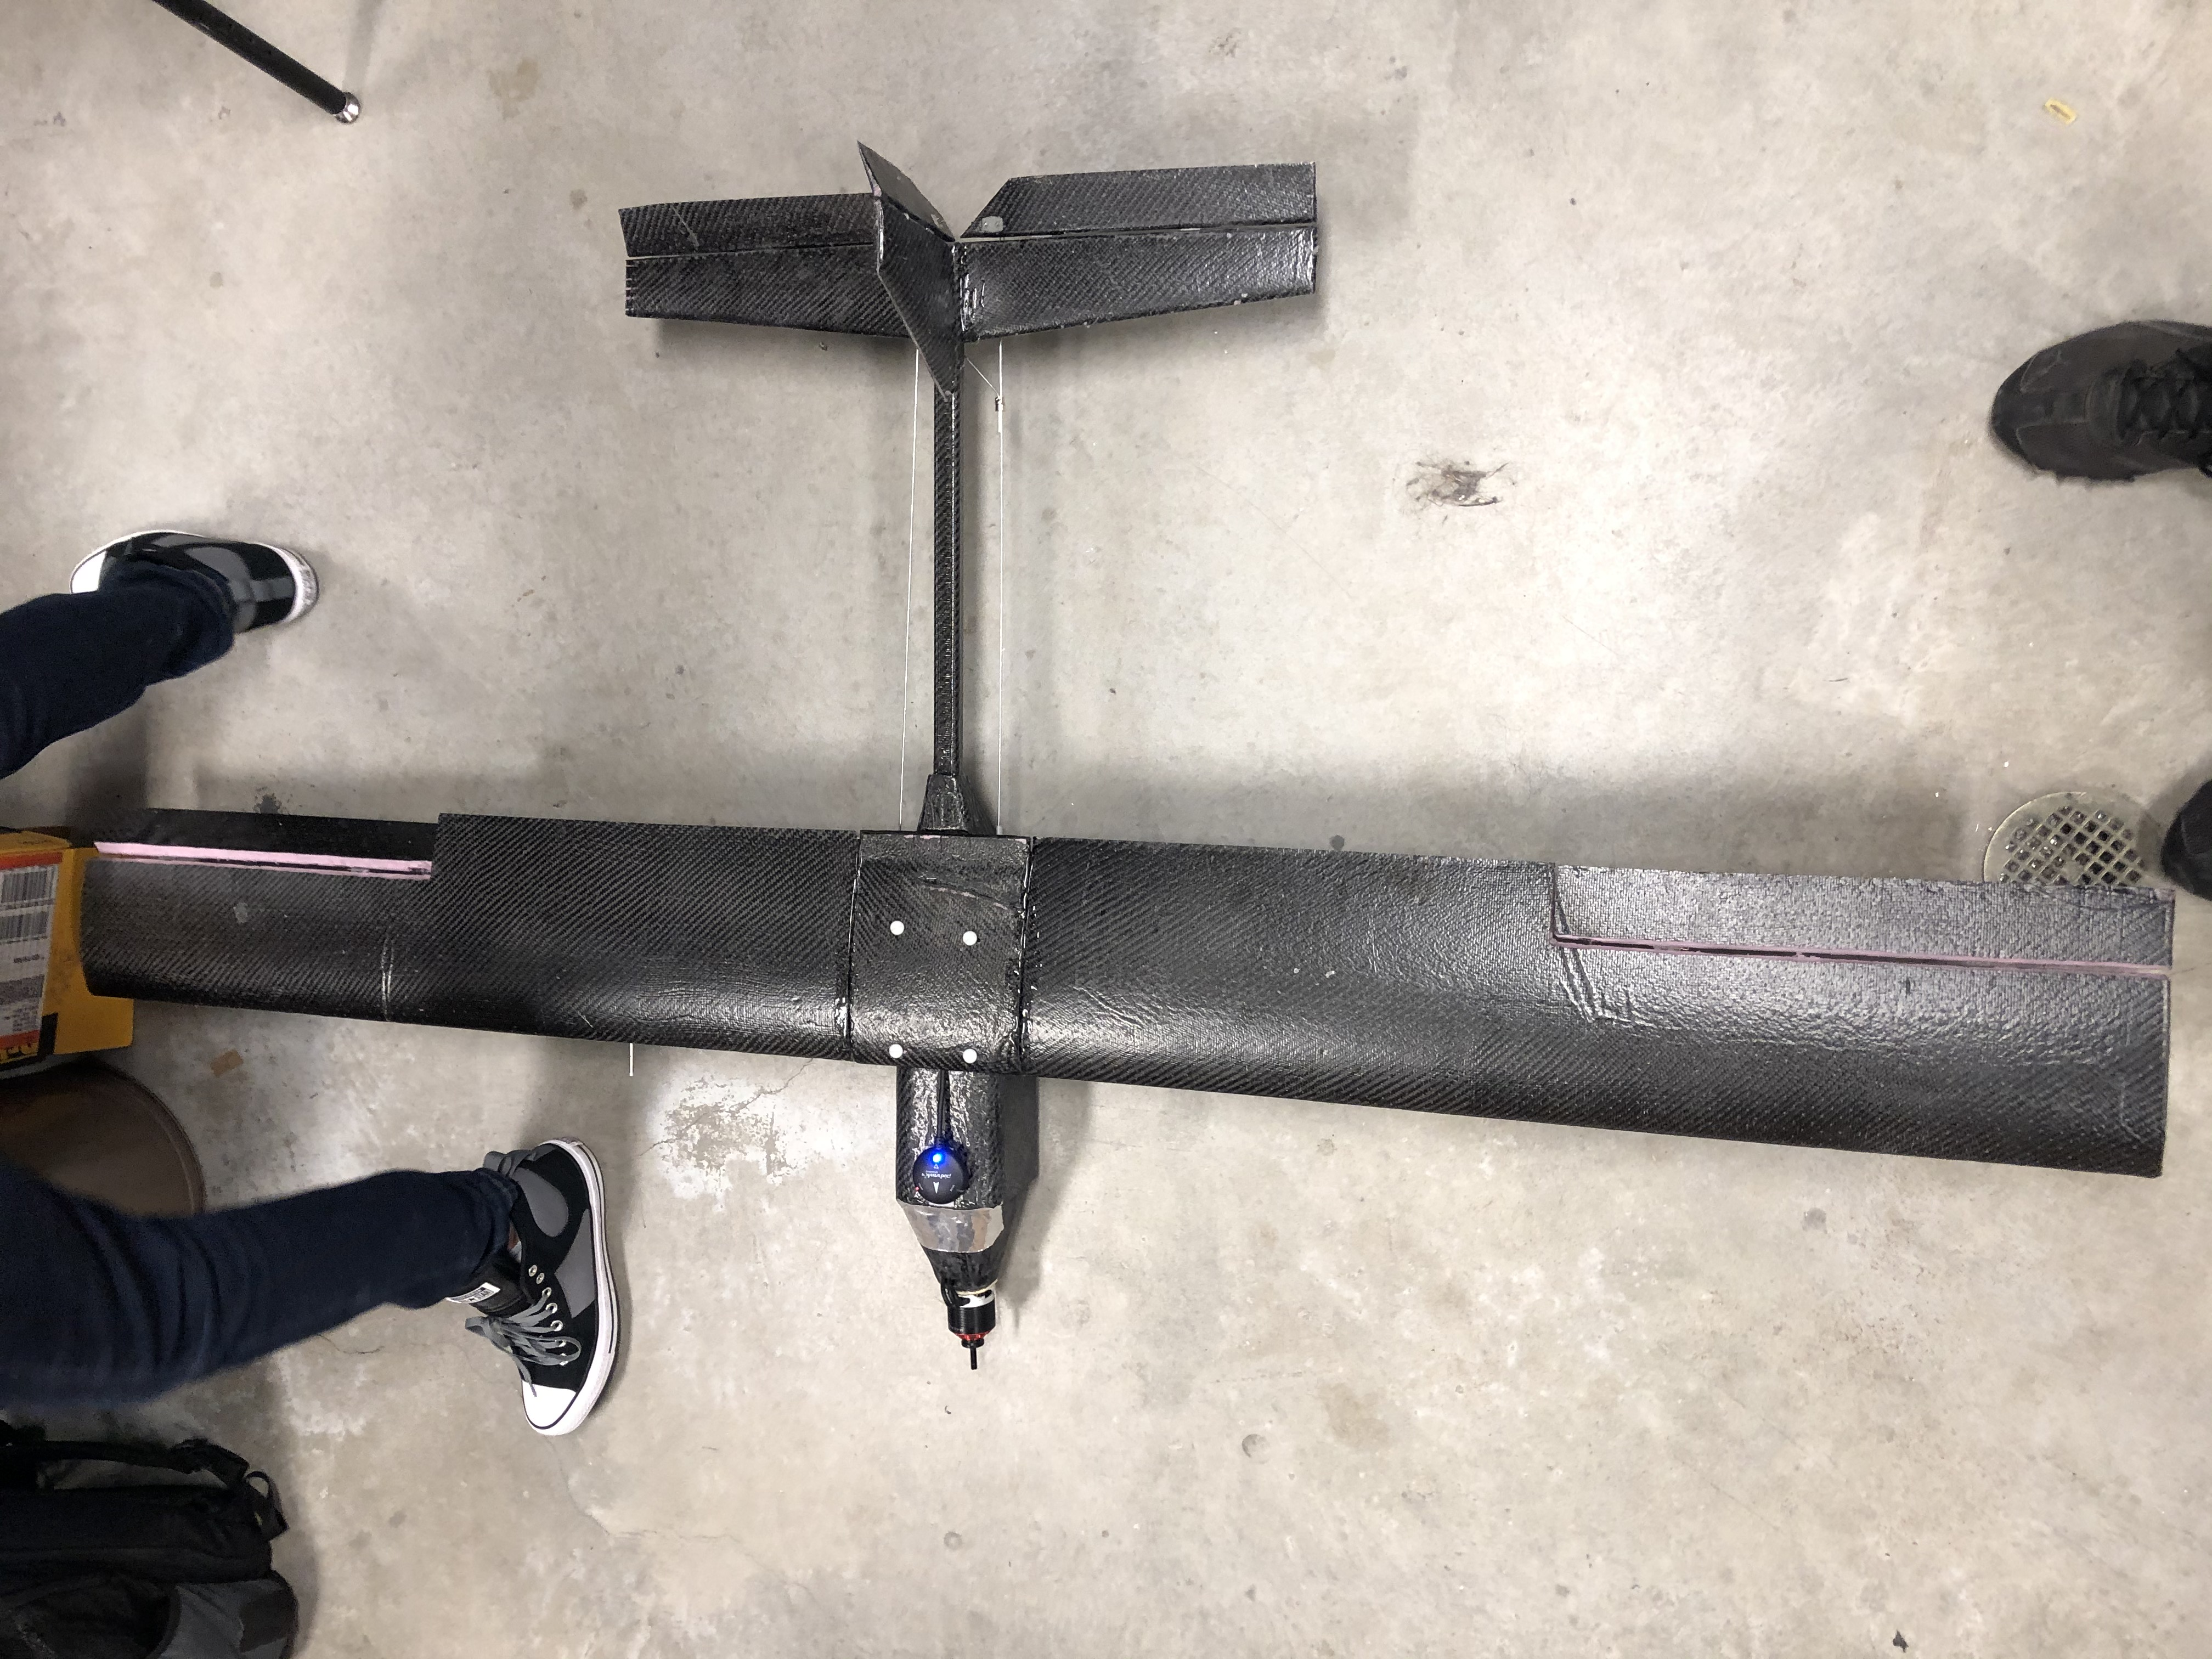
\includegraphics[width = \columnwidth]{UAS_1_0_ImageA.jpg}
	\caption{Assembled UAS 1.0}
\end{figure}

\addcontentsline{toc}{subsection}{Future Work}
\subsection*{Future Work}
List any future work that is planned to be completed based off of this test. \\
\begin{enumerate}
	\item Add landing gear
	\item Increase rudder size
	\item Changing wings to make them lighter / easier to manufacture
	\item Changing tail to make it easier to manufacture and attach it straight
	\item Make electronics bay easier to access
	\item Make manufacturing easier. Carbon fiber is difficult to work with
	\item Reduce costs
\end{enumerate}
\newpage
%Version 1.0 End

%-----------------------------------------------------------------------------------------------------------------------------
\addcontentsline{toc}{section}{UAS 1.1}
\section*{
	\begin{center}
	UAS 1.1
	\end{center}
}

\addcontentsline{toc}{subsection}{Changes}
\subsection*{Changes}
\subsubsection*{Structure Changes}
\begin{enumerate}
	\item Increased rudder size
	\item Added landing gear in tail wheel configuration
\end{enumerate} 
Increasing the rudder size was done to try and increase the control of the UAS and improve the spin recover capability as that is how the UAS 1.0 crashed. Adding the landing gear was done to allow for runway takeoffs and landings. \\ \\

\subsubsection*{Material Changes}
None \\

\subsubsection*{Electronics Changes}
\begin{tabular}{ c c }
	\textbf{Type} & \textbf{Component}  \\ 
	Motor & Badass 2826 - 690KV \\
	Lidar & TF Mini-S
	%Type of Component & Specific Component \\
\end{tabular} \\ \\
This was done to see if using a smaller motor would still allow the UAS to achieve flight. Using a smaller motor will decrease power consumption and thereby increase flight time. The Lidar was added to allow for altitude measuring capabilities which are needed for autonomous landing. \\ \\

\addcontentsline{toc}{subsection}{Tests Performed}
\subsection*{Tests Performed}
What tests if any were performed with this version?
\subsubsection*{Stall Speed Testing}
The UAS was flown in the cardinal directions and speed was gradually reduced until stall was achieved. Because we would then have measurements from all four directions, the average of those values would negate any error from wind speeds. \\
The result of this test was finding that the stall speed is roughly 6 m/s. \\ \\
\subsubsection*{Cruise Speed Testing}
Similarly to Stall Speed Testing, the UAS was flown in the four cardinal directions at cruise speeds and the airspeed was measured. The average was then taken to negate any error from wind speeds. \\
The result of this test was finding that the cruise speed is roughly 20 m/s \\ \\

\addcontentsline{toc}{subsection}{Pilot Comments}
\subsection*{Pilot Comments}
Increasing the rudder size greatly improved the spin recover capabilities. The UAS wanted to roll strongly to the left in flight and took all of the right aileron trim to fly level `hands off'. There were also constant `RF signal low' warnings. Stabilize mode made a huge difference for flight characteristics and helped a lot in making the UAS easier to control.

\addcontentsline{toc}{subsection}{Lessons Learned}
\subsection*{Lessons Learned}
What did we learn from this version? \\ \\
\begin{enumerate}
	\item We needed to have the larger rudder for better control
	\item The smaller motor was more than suffecient for flight, even when using the largest battery
	\item Fuselage may be interfering with RF communications
	\item Something is happening to cause the UAS to want to roll strongly to the left
	\item When doing flight speed or stall tests, keep the UAS in stabilize mode, it helps a lot.
	\item This lidar doesn't sample altitude very quickly which can cause issues in auto landing
\end{enumerate} 

\newpage


%-----------------------------------------------------------------------------------------------------------------------------
\addcontentsline{toc}{section}{UAS 1.2}
\section*{
	\begin{center}
	UAS 1.2
	\end{center}
}

\addcontentsline{toc}{subsection}{Changes}
\subsection*{Changes}
\subsubsection*{Structure Changes}
None \\ \\

\subsubsection*{Material Changes}
 \begin{tabular}{ c c }
	\textbf{Part of UAS} & \textbf{Material}  \\ 
	 Wings & Epoxy Coated Foam  \\  
\end{tabular} \\ \\
This was done to try and make the manufacturing process easier by not needing to use carbon fiber layups. \\ \\

\subsubsection*{Electronics Changes}
\begin{tabular}{ c c }
	\textbf{Type} & \textbf{Component}  \\ 
	Lidar & SF11-C Laser Rangefinder
	%Type of Component & Specific Component \\
\end{tabular} \\ \\
This new lidar should have a faster and more accurate sampling which is needed for recording data and autonomous landing.

\addcontentsline{toc}{subsection}{Tests Performed}
\subsection*{Tests Performed}
What tests if any were performed with this version?
\subsubsection*{Stall Speed Testing}
Stall testing as described in section UAS 1.1 was done again with the UAS in Stabilize and Position mode. This helped to make more accurate data. \\
With this testing, it was found that stall behaviors start occuring at speeds below about 12 m/s. \\ \\
\subsubsection*{Pixhawk Autonomous Control}
In this testing, Stabilize mode and Position mode were tested more thouroughly to try and get accurate data when running other tests. Stabilize mode allows the pilot to control the throttle, but the flight computer will maintain a constant horizontal angle of attack. Position mode tries to maintain a constant heading and altitude if no pilot input is given and will control the throttle as needed to do so. This is very valuable for the stall testing as described above. \\ \\
\subsubsection*{Battery Monitoring}
Updated values were used in the PX4 firmware to allow for more accurate battery monitoring. This was checked in this flight by measuring the voltage before and after attaching the battery, and checking those values against what the QGroundControl software says the real time battery voltage is. \\ 
The result of this test was that the battery voltage monitoring is much more accurate now and can be used to judge when we will be needing to land and switch the battery. \\ \\

\addcontentsline{toc}{subsection}{Pilot Comments}
\subsection*{Pilot Comments}
Overcast sky made it hard to tell which direction the UAS is flying. In future designs, we might want to include color variations to help remedy this. Takeoff is still a challenge. Landing on the grass makes for much better landings and puts the UAS in less danger of ground loops. The epoxy coated wings worked, but they were flexing a lot in flight and it was very concerning.

\addcontentsline{toc}{subsection}{Lessons Learned}
\subsection*{Lessons Learned}
What did we learn from this version? \\ \\
\begin{enumerate}
	\item It is likely the tail that is causing the left-turning issue mentioned before
	\item Add coloring to future UAS versions, hard to tell which way it is flying with cloudy skies
	\item Land on grass when uncertain landing conditions
	\item Steadiness of the wind is moreimportant than wind speed. UAS 1.2 flew well in 10-15 mph winds that were fairly steady.
	\item This lidar sampling was much better and gave more consistent data
\end{enumerate} 

\newpage


%-----------------------------------------------------------------------------------------------------------------------------
\addcontentsline{toc}{section}{UAS 1.3}
\section*{
	\begin{center}
	UAS 1.3
	\end{center}
}

\addcontentsline{toc}{subsection}{Changes}
\subsection*{Changes}
\subsubsection*{Structure Changes}
None \\

\subsubsection*{Material Changes}
 \begin{tabular}{ c c }
	\textbf{Part of UAS} & \textbf{Material}  \\ 
	 Tail Surfaces & Foam  \\  
\end{tabular} \\ \\
The new tail was done to make the manufacturing process easier since it would no longer need carbon fiber layups. \\ \\

\subsubsection*{Electronics Changes}
None \\ \\

\addcontentsline{toc}{subsection}{Tests Performed}
\subsection*{Tests Performed}
What tests if any were performed with this version? \\ \\
None \\

\addcontentsline{toc}{subsection}{Pilot Comments}
\subsection*{Pilot Comments}
Unfortunately, this version was not able to take off. Due to the decreased structural stability in the rudder, the tail wheel had difficulty controling the UAS as it was taking off. In the end, the UAS banked to the left just before takeoff and the bottom part of the rudder snapped off. There are four reasons that generally would cause this turning to the left: P-factor, gyroscopic prescession, torque, and spiraling slipstream. Some things that could help fix this would be angling the motor to counteract the forces or ofsetting the tail or rudder.

\addcontentsline{toc}{subsection}{Lessons Learned}
\subsection*{Lessons Learned}
What other changes would be suggested off of this version? \\ \\
\begin{enumerate}
	\item Rudder will need increased stability
	\item May be worth it to move to a front wheel for the third landing wheel
\end{enumerate}
\newpage



%-----------------------------------------------------------------------------------------------------------------------------
\addcontentsline{toc}{section}{UAS 1.4}
\section*{
\begin{center}
UAS 1.4
\end{center}
}

\addcontentsline{toc}{subsection}{Changes}
\subsection*{Changes}
\subsubsection*{Structure Changes}
\begin{enumerate}
\item Mounted tail wheel to tail boom
\item Added a thin strip of wood to the rudder
\end{enumerate} 
The mounting of the tail wheel was changed to try and make sure it does not break off like it did after the flight test for UAS 1.3. The figure below shows how the wheel was specifically attached: \\
\begin{figure}[H]
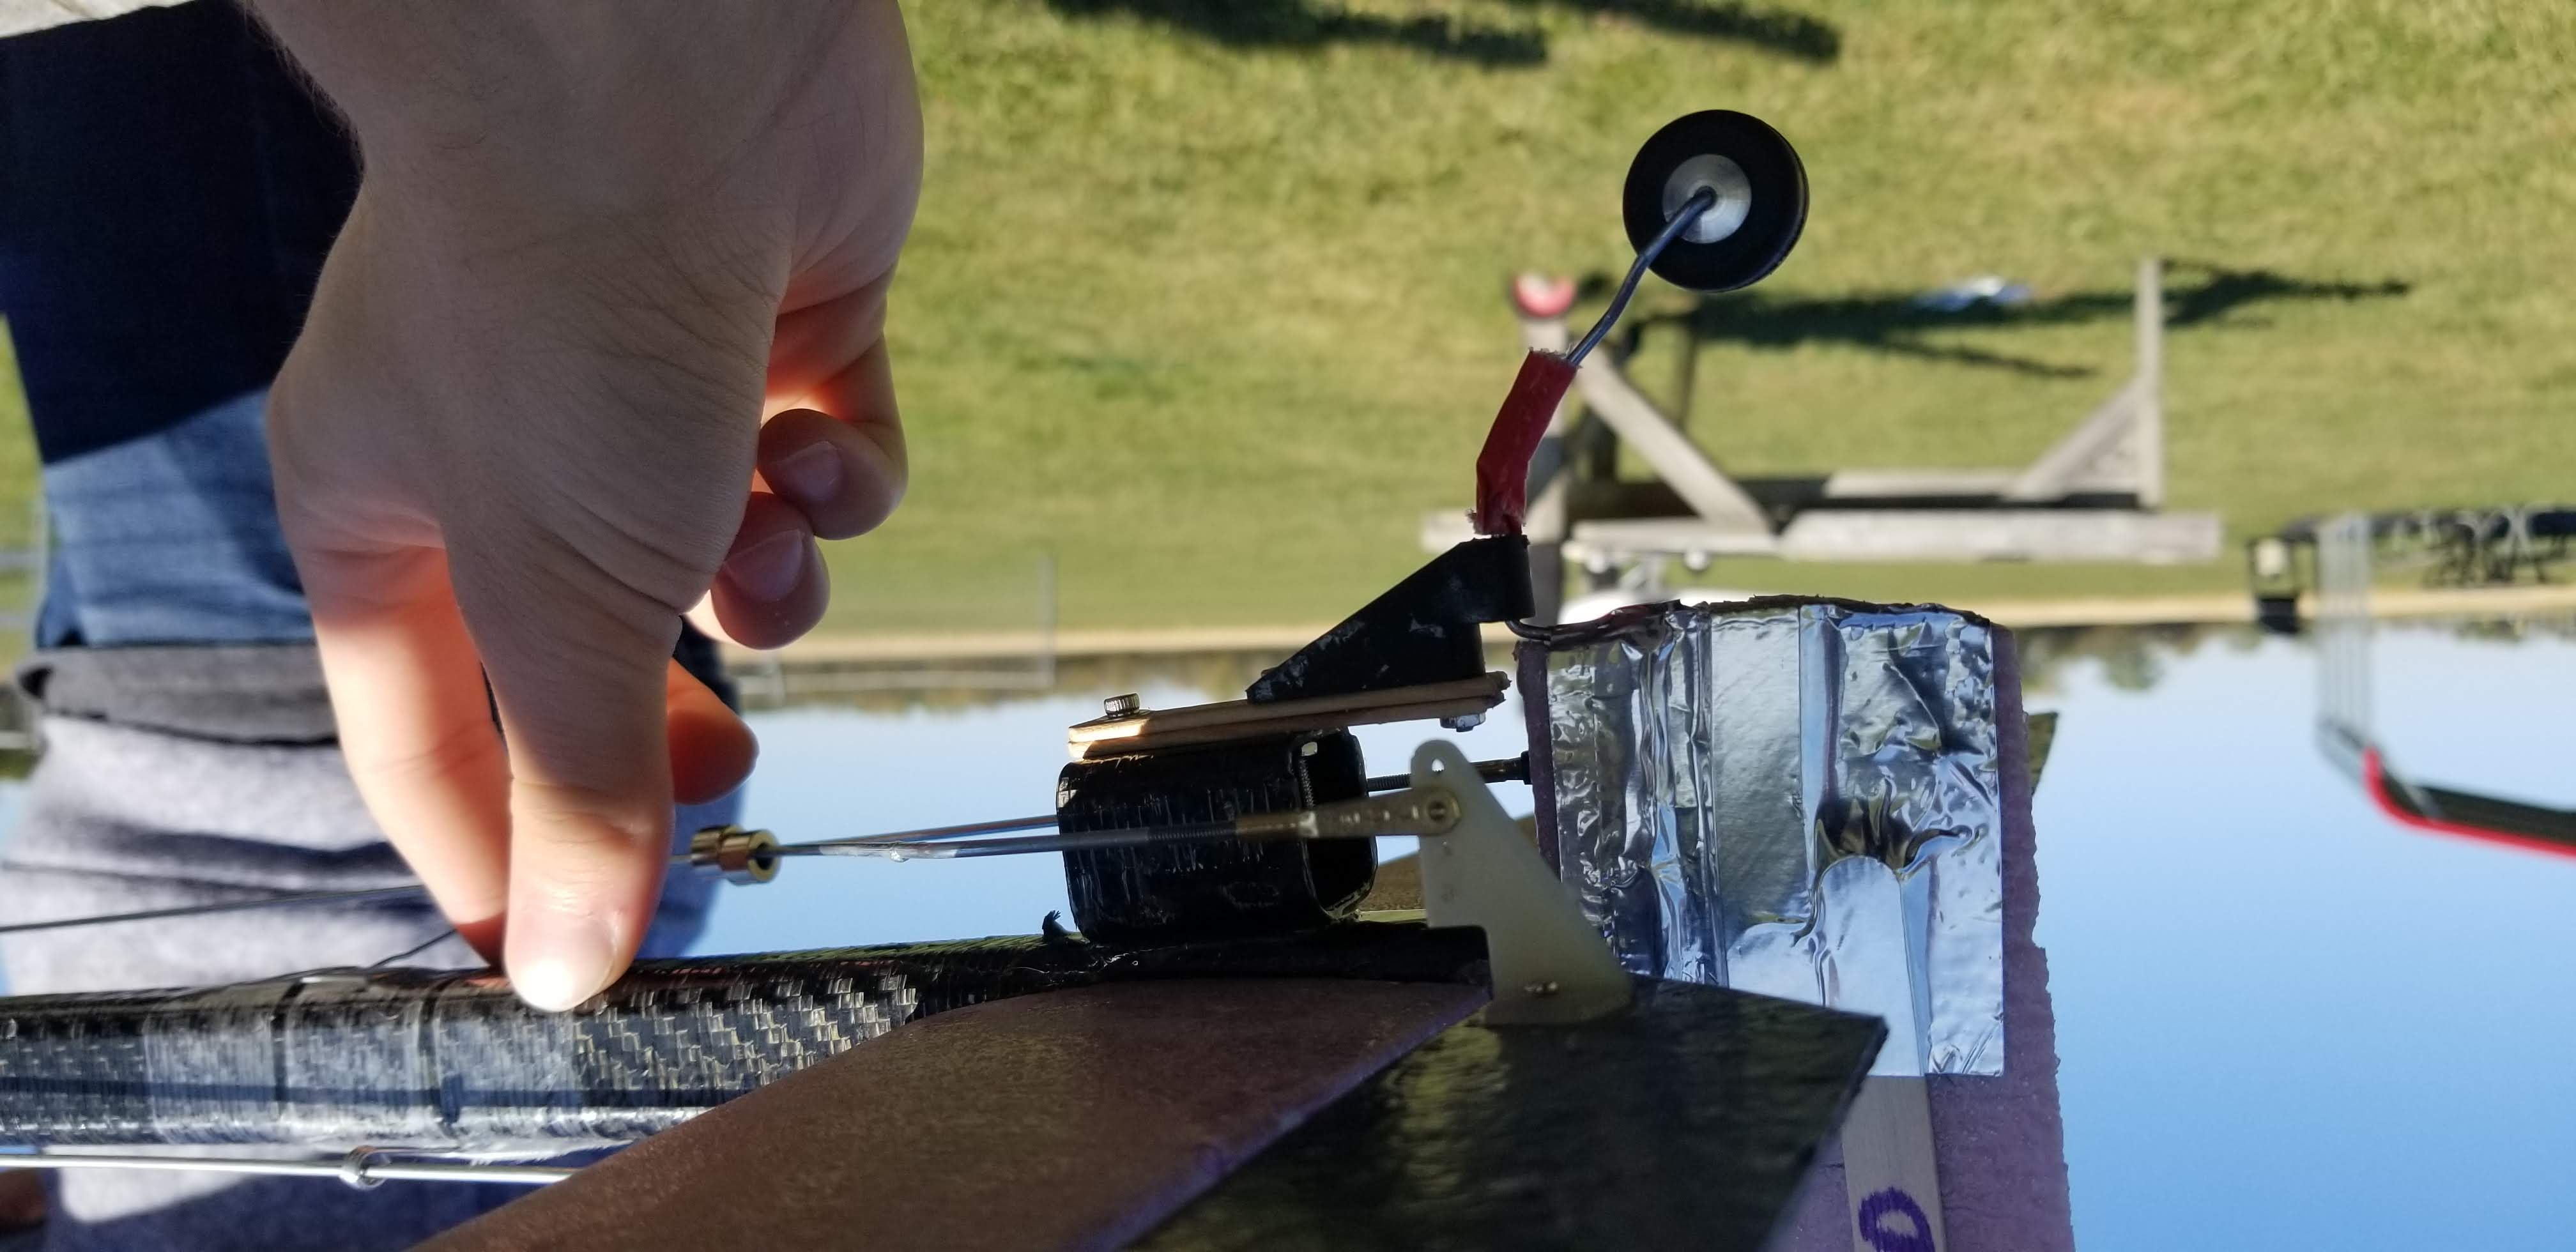
\includegraphics[angle = 180, width = \columnwidth]{UAS1_4_Tailwheel.jpg}
\caption{UAS 1.4 Tailwheel Mounting}
\end{figure}

The thin strip of wood was added to the rudder in order to stiffen the foam so that it does not break as happened in the UAS 1.3 test flight. The construction of this stiffener is shown below: \\
\begin{figure}[H]
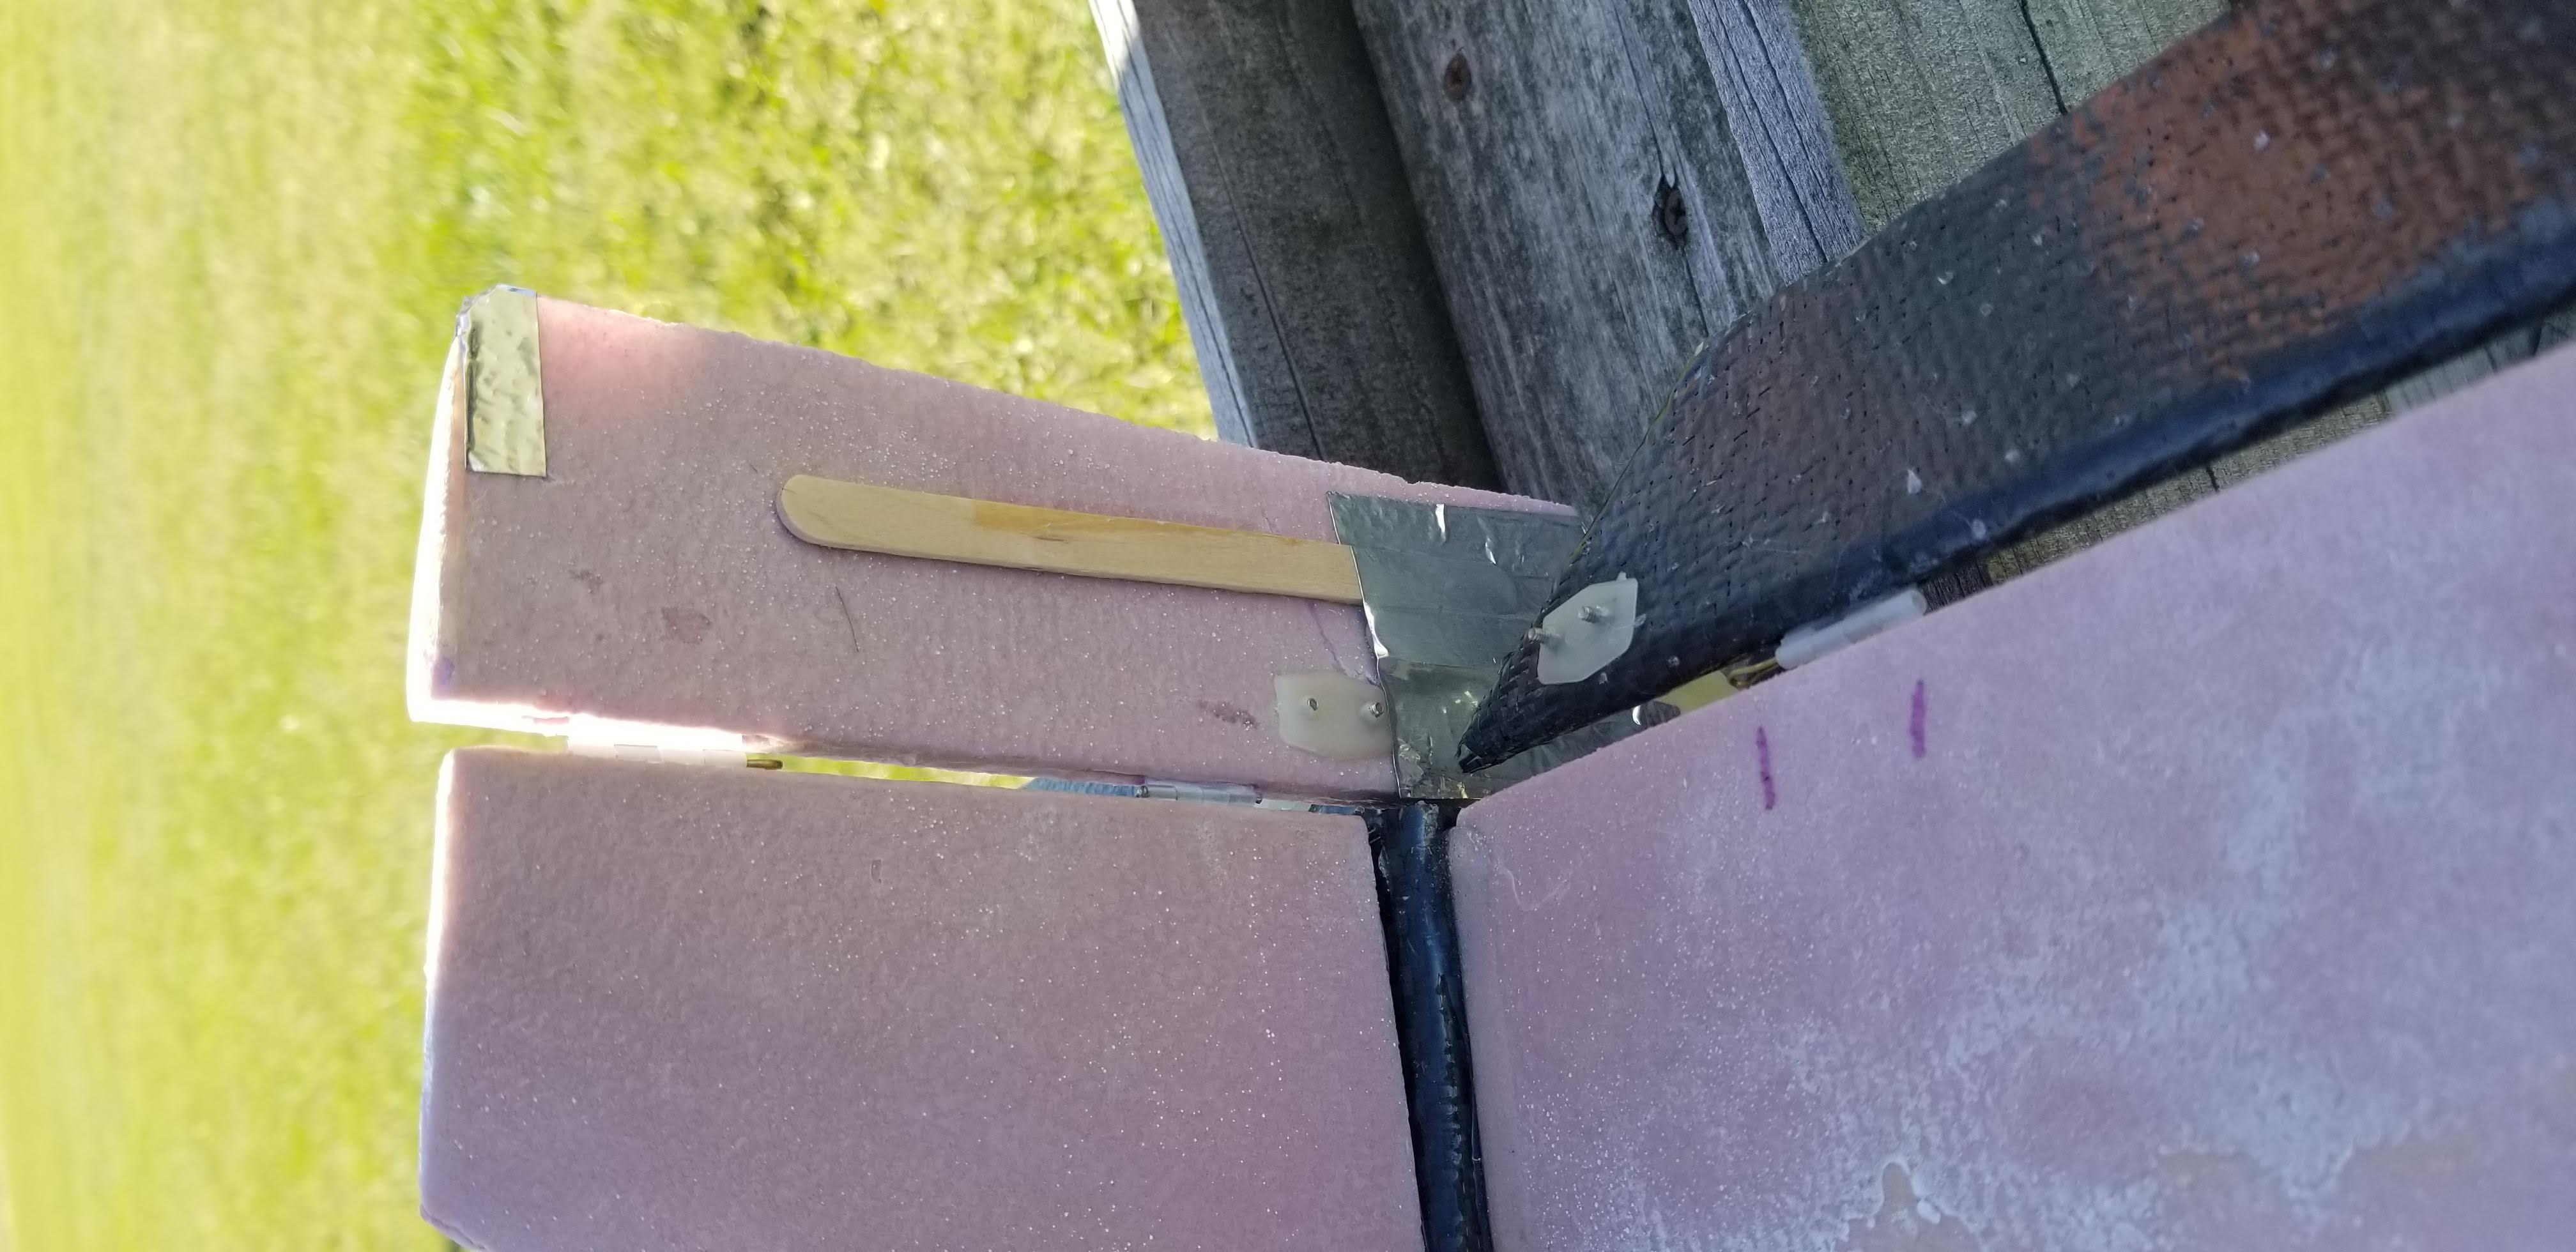
\includegraphics[angle = 270, width = 5cm]{UAS1_4_RudderStiffener.jpg}
\caption{UAS 1.4 Rudder Stiffener}
\end{figure}


\subsubsection*{Material Changes}
\begin{tabular}{ c c }
\textbf{Part of UAS} & \textbf{Material} \\ 
Tail Surfaces & Foam \\ 
Wings & Foam with Monokote Wrap and Carbon Fiber Stiffener Rods \\
\end{tabular} \\ \\ \\
The new tail was done to make the manufacturing process easier since it would no longer need carbon fiber layups. This is the same tail that was being tested in UAS 1.3 with the structure changed noted above to prevent the same failures from happening. The wings were made to help make manufacturing easier as well. The carbon fiber stiffeners and monokote were used on top of the foam to give it more strength and prevent the large wing deflections that were seen when using the solid foam wing in UAS 1.2. \\ \\

\subsubsection*{Electronics Changes}
None \\ \\

\addcontentsline{toc}{subsection}{Tests Performed}
\subsection*{Tests Performed}
What tests if any were performed with this version?
\subsubsection*{Full Autonomous Mission - Apprentice}
In this test, the aim was to use a commercially available UAS (E-Flight Apprentice) and run a full mission completely autonomously. The same firmware was used as is used on the OpenUAS. First, the Apprentice was hand launched, then it would follow a path to a number of previously set waypoints, and finally, it would autonomously land. \\
The autonomous takeoff went very smoothly and the Apprentice was able to correct itself and travel to the waypoints. As the Apprentice was approaching for landing, about 10-15 feet above the runway, it aborted. There was almost no wind and the line up for landing seemed perfect. It is predicted that this occured due to insufficient data. The Apprentice does not have an integrated Lidar sensor to determine the altitude. The OpenUAS does have this sensor, so in future tests, adding this sensor may allow the Apprentice to autonomously land. \\ \\

\subsubsection*{Foam Tail Performance}
In this test, the aim was to fly the UAS 1.4 and observe how it handles differently after changing the tail from carbon fiber layups to only foam tail pieces. The wing used was the one with carbon fiber layups. Before flight, all software and controls were checked and verified to be accurate. A taxi test was also performed to verify the movement and response of the UAS at low speeds. This taxi test showed that the new mounting of the tail wheel was successful and held up during movement on the ground. \\
During takeoff, as the UAS accelerated and was just beginning to get off the ground, there was an intense left yawing. This caused the craft to spiral to the left and eventually impact the ground. After examining the data, it seems that the stabilize mode that the UAS was in was trying to correct for this yaw and that the servos were responding properly. The only explanation that we can find for this left yaw at this point is due to the torque of the motor. In future tests, we plan to fix this by angling the motor to the right. \\ \\

\subsubsection*{Hand Launch Test}
In this test, we wanted to confirm the left yawing that we saw in the previous test. Because the landing gear broke off on impact of the previous test, the craft was repaired as best possible in the field and an autonomous hand launch was used. The repairs done are shown in the figure below.
\begin{figure}[H]
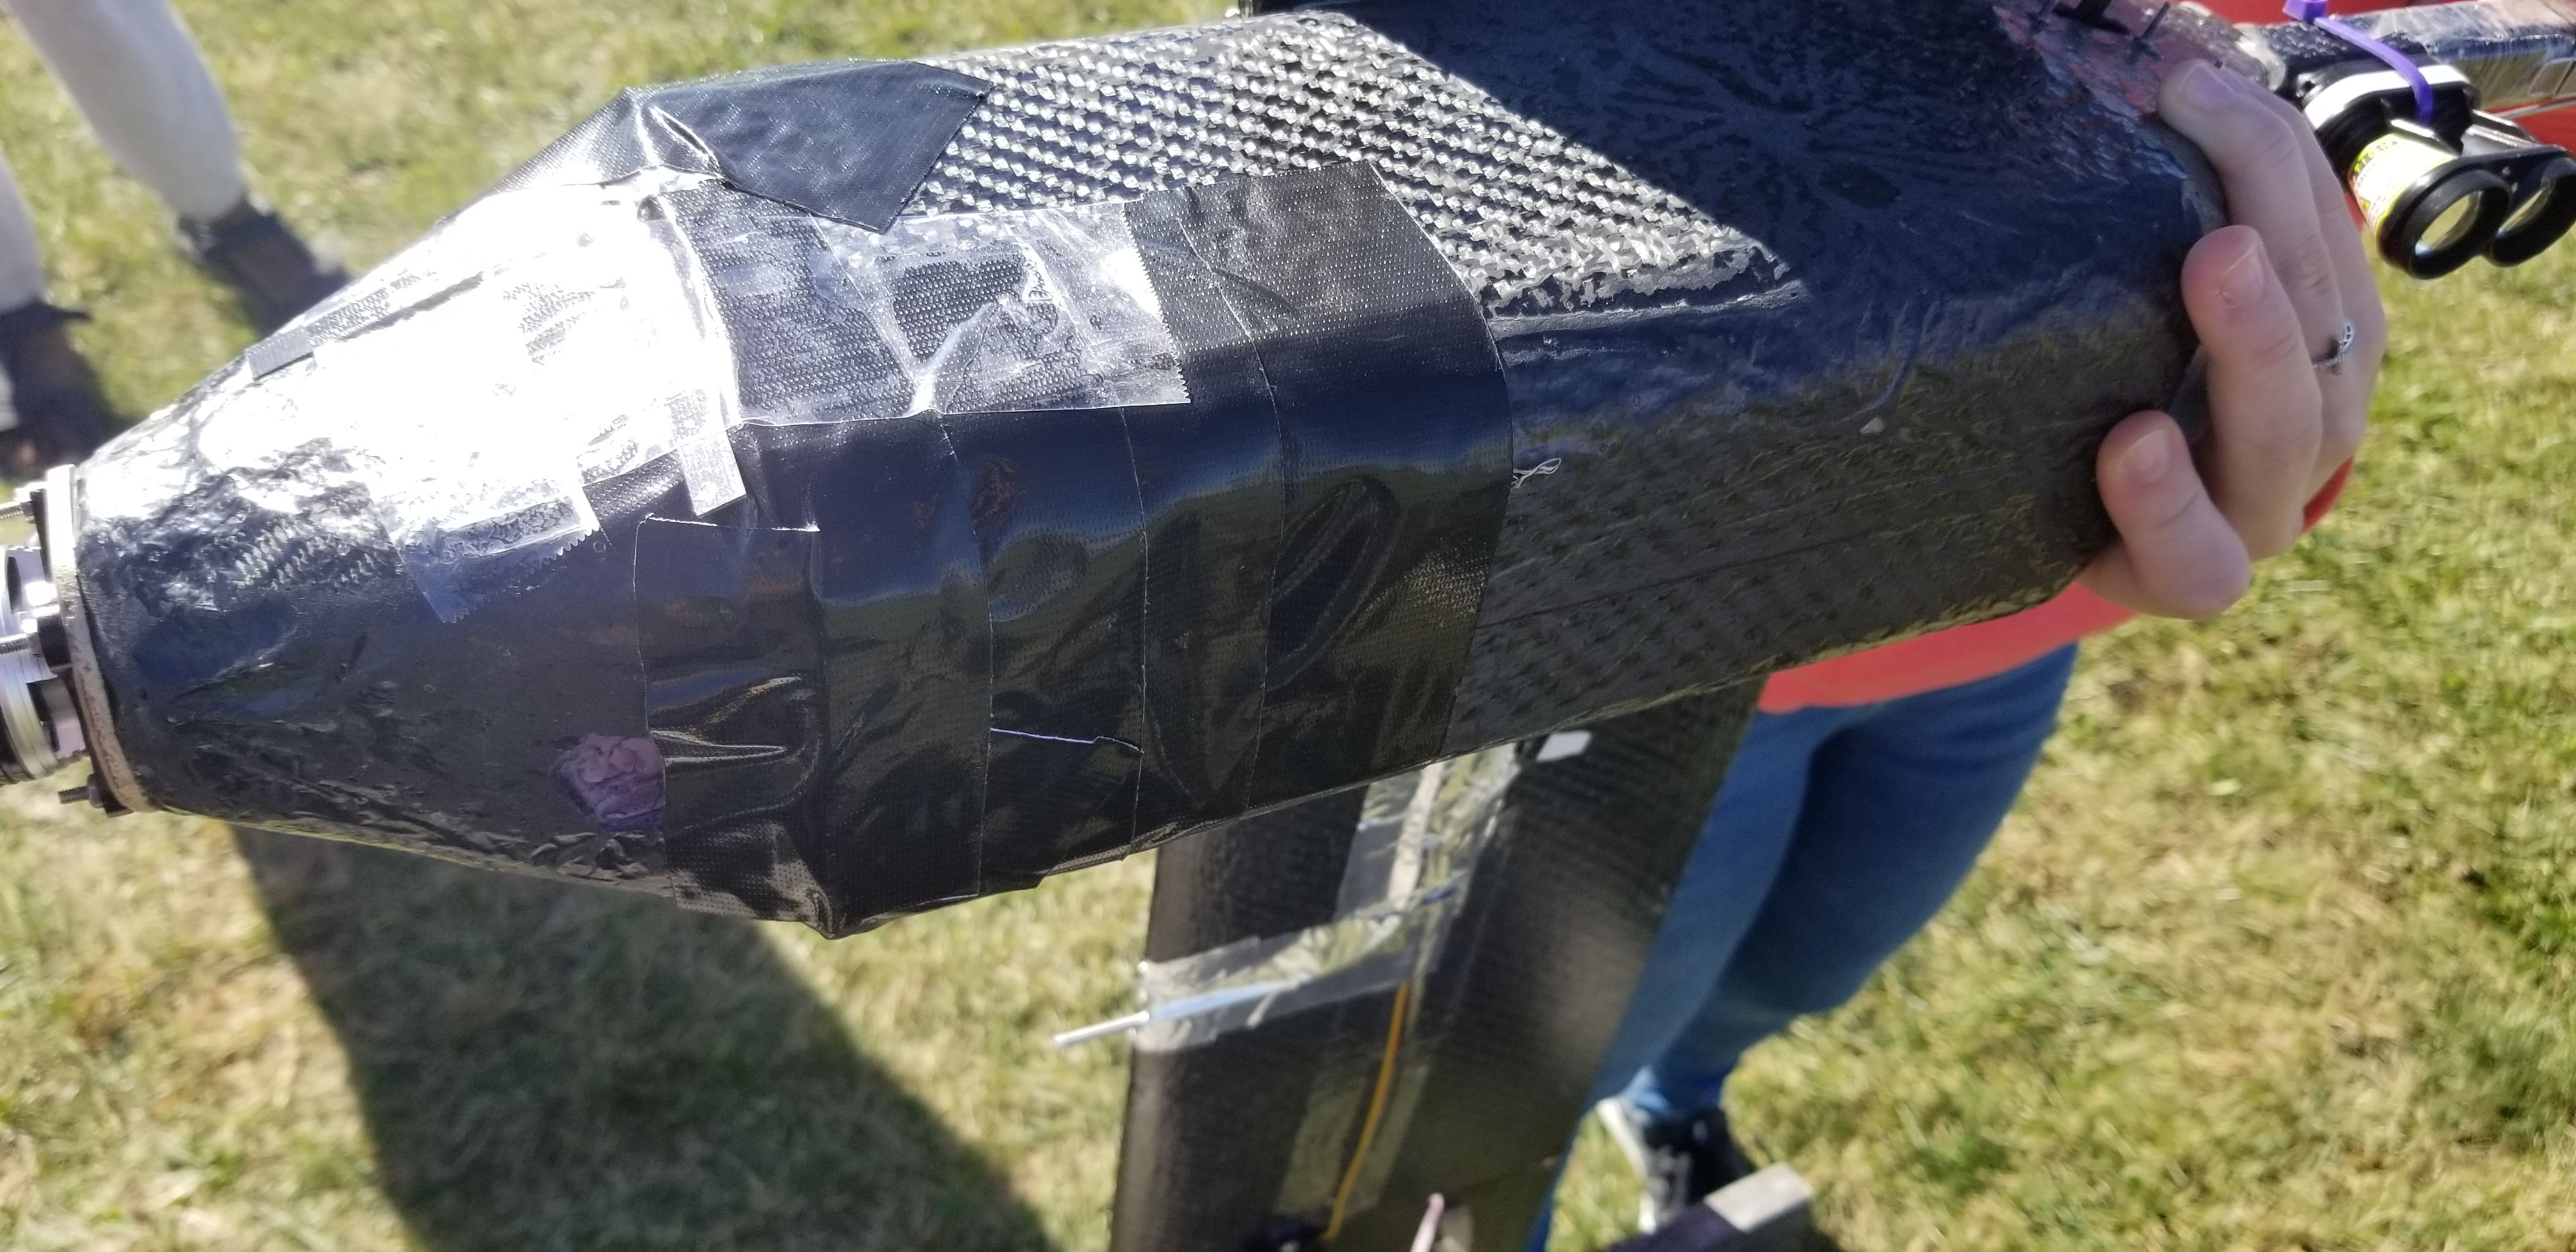
\includegraphics[width = \columnwidth]{UAS1_4_RepairsB.jpg}
\caption{UAS 1.4 Fuselage Repairs}
\end{figure}

The mission uploaded was the same mission that was used successfully on the Apprentice in the first test of this version, so the performance up until the landing had been verified. After the initial hand launch, the craft climbed and took off as expected, but quickly started to yaw to the left again and eventually fell and crashed. This test verified that it was not a software / firmware issue that was causing this yawing response. \\ \\

\subsubsection*{Monokote Wing Performance - Apprentice}
In this test, the monokote wing with carbon fiber stiffener rods was tested. Since the OpenUAS was broken beyond repair after the previous test, the wing was attached to the Apprentice fuselage as shown below:
\begin{figure}[H]
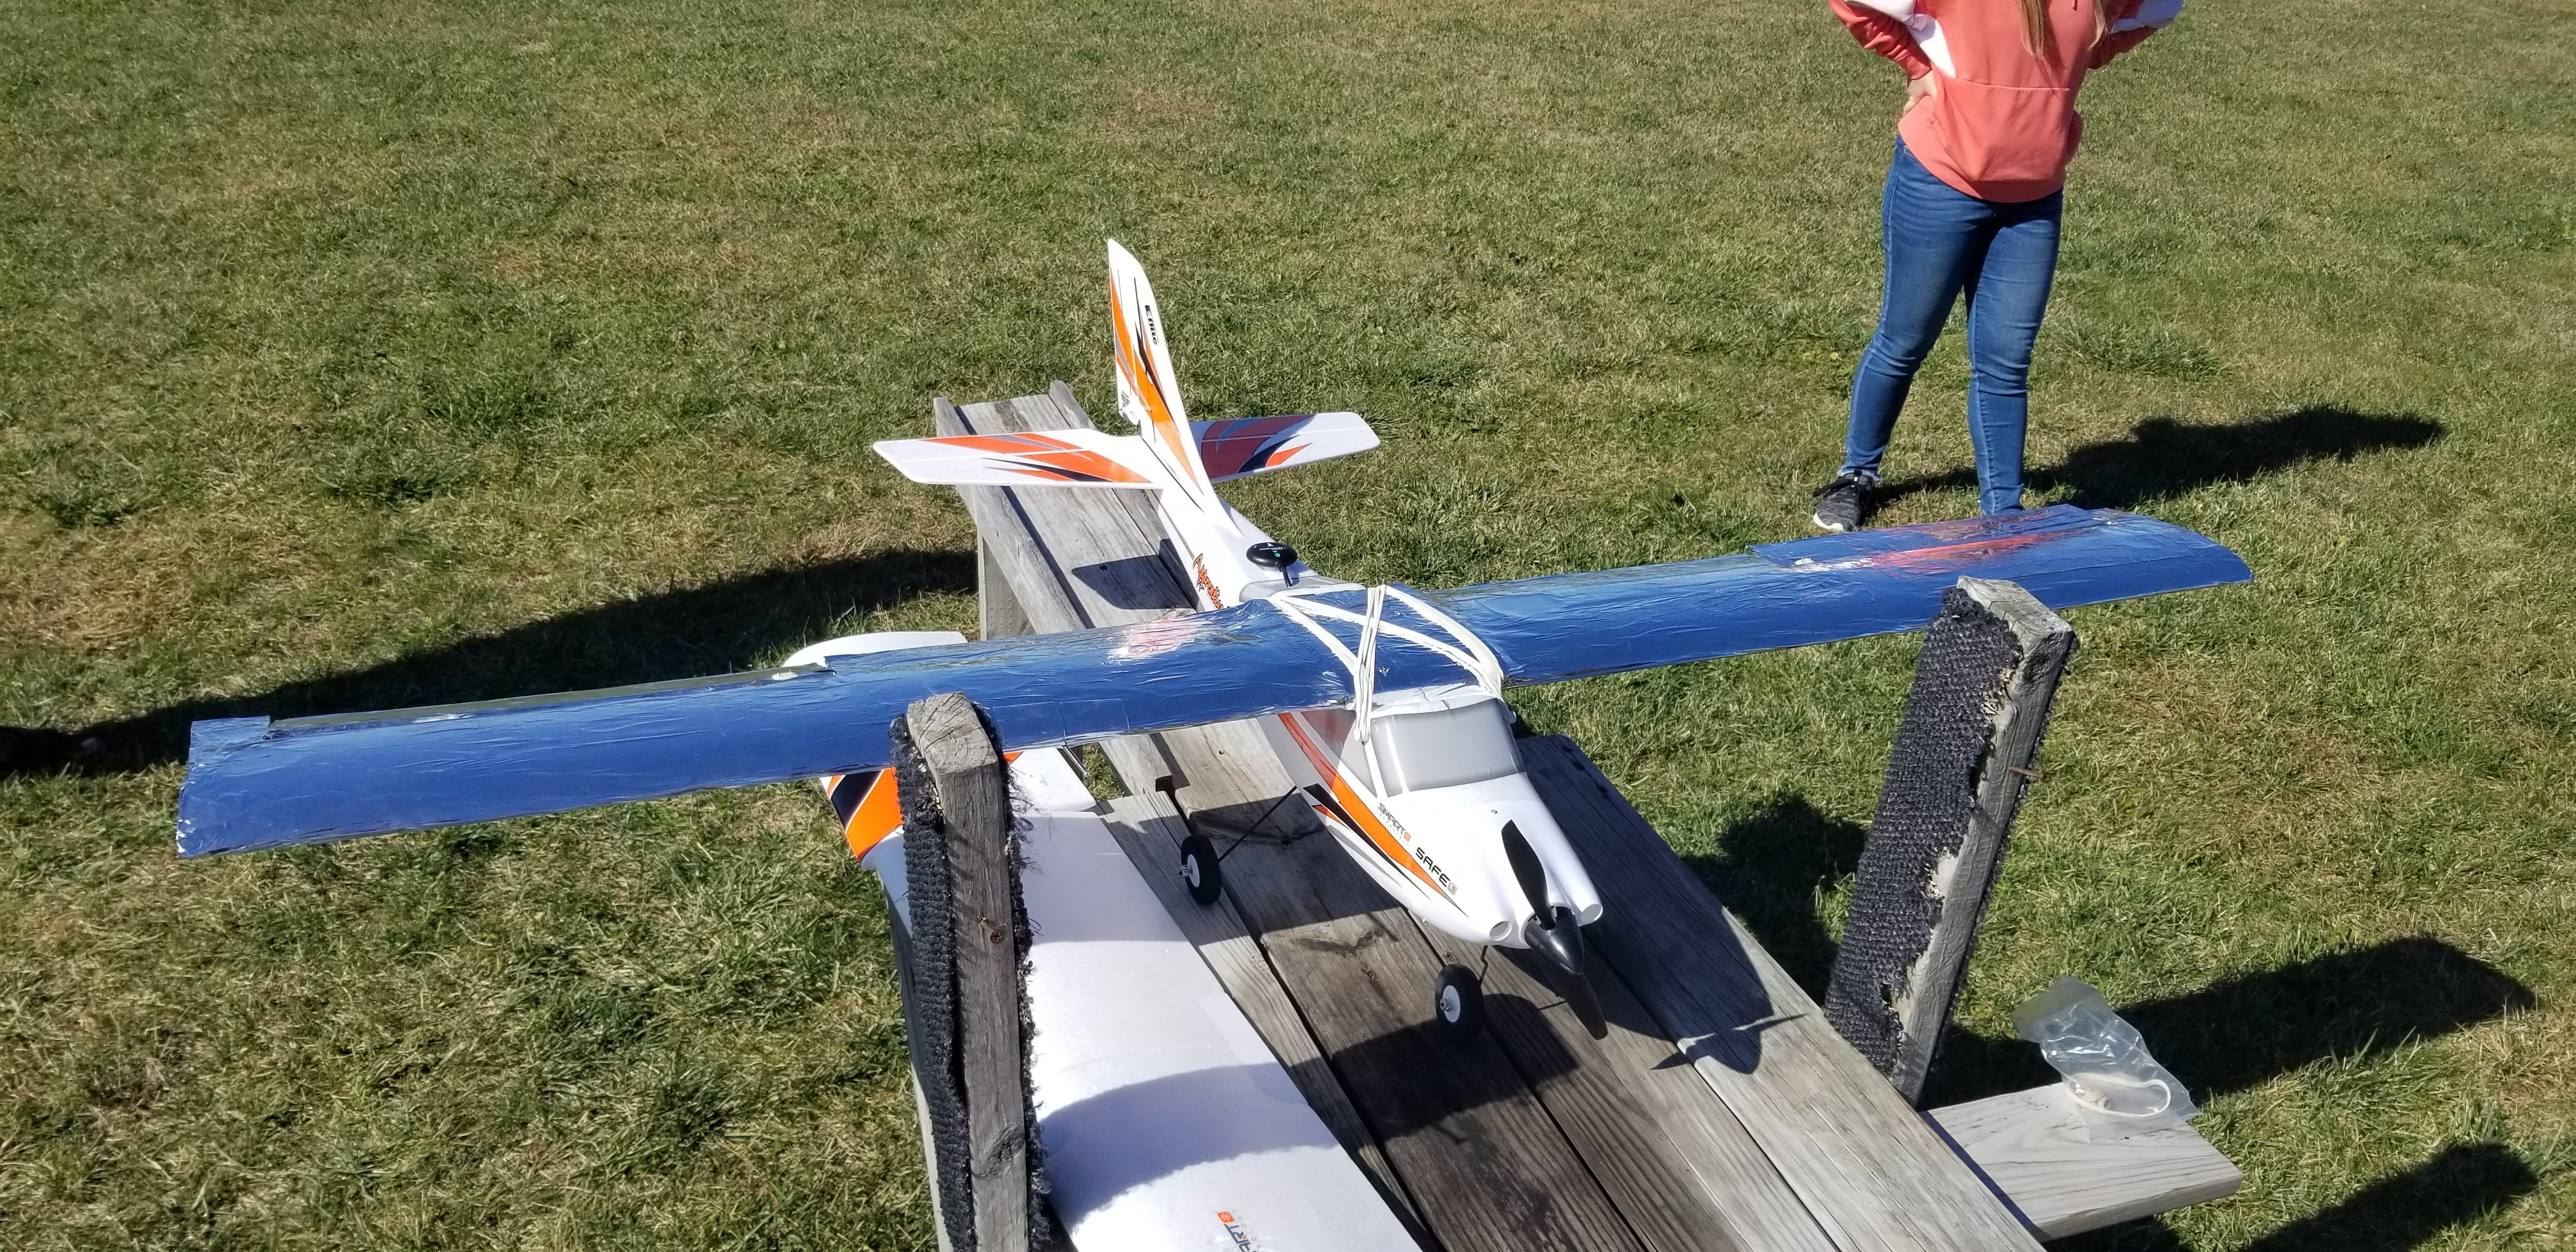
\includegraphics[width = \columnwidth]{Apprentice_MonokoteWing.jpg}
\caption{E-Flight Apprentice with Monokote Wing attached}
\end{figure}
The purpose of this test was to check if adding the stiffener rods and the monokote helps to prevent flexing and failure of the mainly foam wing. This test did a manual runway takeoff and then tested the responses of the Apprentice when flying, the flexing of the wing during rapid elevator deflections, and stall characteristics of the wing. \\
The takeoff was performed in stabilize mode, the same mode that the Foam Tail Performance test was started in, to further ensure that it was not a firmware issue causing the OpenUAS yawing. the Apprentice took off and flew smoothly. Roll responses were slightly reduced, but that is to be expected because the Monokote wing is longer than the original wing for the Apprentice. During stall testing, the Apprentice stalled at about 5 m/s and then would slowly glide downwards, but was easy to recover. The wing did flex considerably during rapid pitch changes, but there wasn't a concern of breakages as there was with the purely foam wing due to the added carbon fiber rods. \\

\addcontentsline{toc}{subsection}{Pilot Comments}
\subsection*{Pilot Comments}
For the first flight with the actual UAS, it displayed the same yawing characteristics observed in the UAS 1.3. Due to the early crash, not much data was able to be obtained, but the tail wheel was decisively off the runway before the yawing started, so a weak tail wheel can be ruled out as a cause for this issue. For the hand launch, the UAS took off as expected but stil displayed the same characteristic as it leveled off. By further testing of the software, bugs there were able to be ruled out as well, leaving the cause to lie in the structure or other physical aspects of the craft. \\
Testing the foam wing on the Apprentice helped to show the wing capabilities going forward. There was a considerable amount of flex in the wing during flight which created a dihedral, even though that wasn't inherintly present in the wing design. Even though the wing flexed, it was less than the pure foam and epoxy wing and it didn't seem in danger of breaking. This was due to the added carbon fiber rods. This would be a good wing composition going forward.

\addcontentsline{toc}{subsection}{Lessons Learned}
\subsection*{Lessons Learned}
What other changes would be suggested off of this version? \\ \\
\begin{enumerate}
	\item Pitot tube needs to be calibrated a lot. Are there good ways to fix this?
	\item Carbon Fiber Stiffener rods seemed to help the foam wings a lot
	\item Mount the motor at an angle to the right, this may help the yawing issue
	\item Build a test stand to check for this yawing issue statically before flight tests
	\item Test adding a Lidar to Apprentice or future UAS to test autonomous landing with more data
	\item Autonomous hand launching works very well when a runway is not available
	\item Silver monokote is very hard to see when flying
\end{enumerate} 



\end{document}
